\documentclass[a4paper,12pt]{article}

\usepackage[]{geometry} 
\usepackage{graphicx}
\usepackage{graphics}
\usepackage{amsmath}
\usepackage{url}
\usepackage{float}
\usepackage{hyperref}
\usepackage{listings}
\usepackage{minted}
\usepackage{pdflscape}
\usepackage{rotating}
\usepackage{mdframed}
\usepackage{wrapfig}
\usepackage{bm}
\usepackage{subcaption}
%\usepackage{fontspec}

\hypersetup{ colorlinks=true, linkcolor=blue, filecolor=magenta, urlcolor=cyan }
\renewcommand\listoflistingscaption{List of source codes}
%\setmonofont{Consolas}

\begin{document}
	
\begin{titlepage}
	\title{
		COMP6223 Computer Vision \\
		\large Image Filtering and Hybrid Images
	}
	\date{\today}
	\author{
		Ganiyu Ajibola Ibraheem \\
		\large gai1u17@soton.ac.uk \\
			29447267
	}
\end{titlepage}

\maketitle
\newpage
\pagenumbering{roman}
\tableofcontents
\newpage
\listoffigures
\listoftables
\listoflistings
\newpage
\pagenumbering{arabic}


\section{Convolution and Hybrid Images Algorithm}
% In the report you need to describe your convolution and hybrid images algorithms (in particular, please include your code for the convolution implementation)
\begin{figure}[h!]
	\centering
	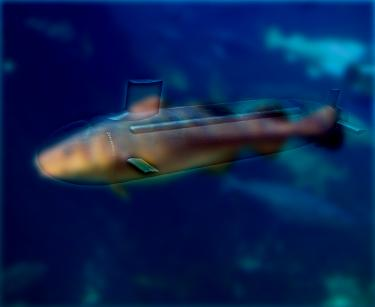
\includegraphics[width=0.35\linewidth]{images/fish_submarine}
	\caption{Hybrid Image of a fish and a submarine}
	\label{fig:fish_submarine}
\end{figure}
The convolution algorithm can be used to generate an hybrid image as shown in figure \ref{fig:fish_submarine} and it works for any arbitrary image and a given odd numbered kernel size. \\

The hybrid image algorithm works in 3 parts which are reading in the images, finding the high frequencies and low frequencies of the images and lastly combining them to form an hybrid image. The algorithm was implemented using Matlab and its implementation are further discussed in the following subsections.

	\subsection{Reading in the Images}
	Matlab provides functions for reading in images which is the \textit{imread} function. 
	\begin{listing}[htbp!]
		\inputminted[breaklines=true,breakautoindent=true,firstline=9,lastline=14]{matlab}{minty_matlab.m}
		\caption{Reading in an image and separation of channels}
		\label{code:algebraic} 
	\end{listing}
	The images are read and converted into doubles as they are stored as integers and need to be converted to work in Matlab.
	
	\subsection{Determining the Low and High Frequencies of the Image}
	The Low frequency of the image is determined by generating a Gaussian kernel of a specified size. For a given kernel size e.g 7x7, with variance ($\sigma^2$) the resulting Gaussian Kernel is calculated by 
		\begin{equation}
			gaussian(x,y) = \frac{1}{\sqrt{2\pi\sigma^2}}\exp-\frac{x^2 + y^2}{2\sigma^2}
		\end{equation} 
	The convolution of the Gaussian kernel and the image produce a low frequency image as shown in figure \ref{fig:low_ein}. The high frequency of the image is obtained by subtracting the low frequency from the original image and an example is shown in figure \ref{fig:high_freq}.
	\begin{figure}[h!]
		\centering
		\begin{subfigure}{0.4\textwidth}
			\centering
			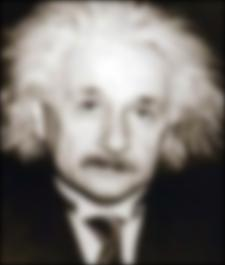
\includegraphics[width=0.99\linewidth]{images/low_freq_ein}
			\caption{Low Frequency Image}
			\label{fig:low_ein}
		\end{subfigure}
		\begin{subfigure}{0.4\textwidth}
			\centering
			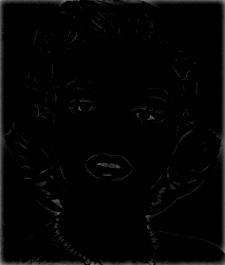
\includegraphics[width=0.99\linewidth]{images/high_freq_mar}
			\caption{High Frequency Image}
			\label{fig:high_freq}
		\end{subfigure}
		\caption{High and Low Frequency Image}
		\label{fig:uni_gauss}
	\end{figure}
	The image convolution code is further show in 
% Any decisions you made to write your algorithms in a particular way. 
\section{Results}
% Then you should show and discuss the results of your algorithm, showing the results of your hybrid images algorithm (showing the image at a range of scales to show the effect)
% show some of the intermediate images in the hybrid image pipeline (e.g. the low and high frequency images). 
\section{Conclusion}
% Also, discuss anything extra you did. Feel free to add any other information you feel is relevant.



\end{document}